\documentclass[12pt, a4paper, onecolumn]{exam}
\usepackage{amsmath}
\usepackage{amssymb}
\usepackage{graphicx}
\usepackage{pdfpages}
\usepackage[linesnumbered,ruled]{algorithm2e}
\graphicspath{ {./images/} }
\usepackage[lmargin=71pt, tmargin=1.2in]{geometry}  %For centering solution box
% \lhead{Leaft Header\\}
% \rhead{Right Header\\}
% \chead{\hline} % Un-comment to draw line below header
\thispagestyle{empty}   %For removing header/footer from page 1

\usepackage{tcolorbox}
\tcbuselibrary{theorems}

\newtcbtheorem[number within=section]{theo}{Theorem}%
{colback=green!5,colframe=green!35!black,fonttitle=\bfseries}{th}

\newtcbtheorem[number within=section]{hypothesis}{Hypothesis}%
{colback=red!5,colframe=red!35!black,fonttitle=\bfseries}{th}

\newtcbtheorem[number within=section]{define}{Definition}%
{colback=blue!5,colframe=blue!35!black,fonttitle=\bfseries}{th}

\newcommand{\RP}{\ensuremath{\mathsf{RP}}}
\newcommand{\expect}[1]{\ensuremath{\mathbb{E}[#1]}}
\newcommand{\dx}{\mathrm{d}x}
\newcommand{\NP}{\ensuremath{\mathsf{NP}}}
\newcommand{\co}{\ensuremath{\mathsf{co}\mbox{-}}}
\newcommand{\NL}{\ensuremath{\mathsf{NL}}}

\begin{document}

\hrule
\vspace{1em}

\begingroup
\centering
\large \textsc{Probabilistic and Smoothed Analysis of Algorithms}\\
\large \textsc{End Semester Examination}\\[0.5em]
\large \today\\[0.5em]
\large \textsc{Roy, Akash} $\mid$ CS22M007\par
\large \textsc{M.Tech CS} $\mid$ \textsc{Indian Institute of Technology, Madras}\par
\endgroup
\pointsdroppedatright %Self-explanatory
\printanswers
\renewcommand{\solutiontitle}{\noindent\textbf{Ans:}\enspace}   %Replace "Ans:" with starting keyword in solution box

\vspace{1em}
\hrule
\vspace{0.2em}

\begin{center}
	\textsc{Answering any} $4$ Question.
\end{center}

\vspace{0.2em}
\hrule
\vspace{1em}

\begin{questions}

    \question Question 1 from Probabilistic Analysis

    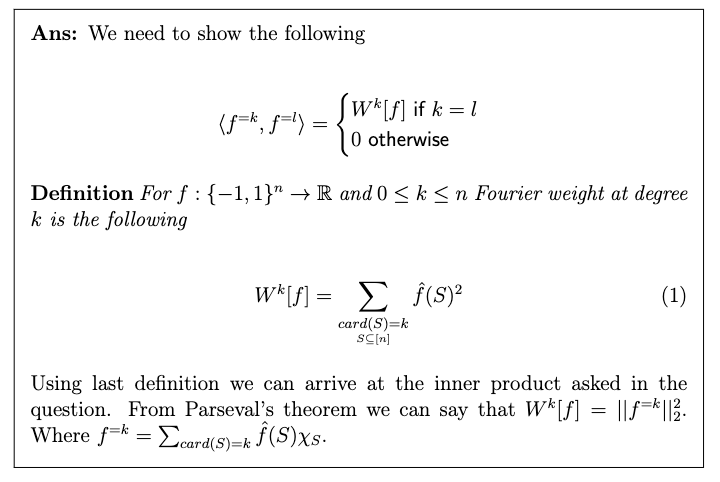
\includegraphics[]{question1}
    
    \begin{solution}
        
    \end{solution}

\end{questions}
\end{document}